See  
\figref{fig:chapters/12/10/5/3Fig1}.
Let the initial position
be
\begin{align}
	\vec{A}=\myvec{0\\0}
\end{align}
After going west, the position becomes
\begin{align}
			\vec{B}=\myvec{-4\\0}
\end{align}
If the final position be $\vec{C}$, from the given information,
\begin{align}
	 \vec{C}-\vec{B}=3\myvec{\cos{60\degree}\\\sin{60\degree}}
	 \implies 
	\vec{C}  
=\myvec{\frac{-5}{2}\\[2pt] \frac{3\sqrt{3}}{2}}
\end{align}
which is the desired displacement. 
\begin{figure}[H] 
 \begin{center} 
 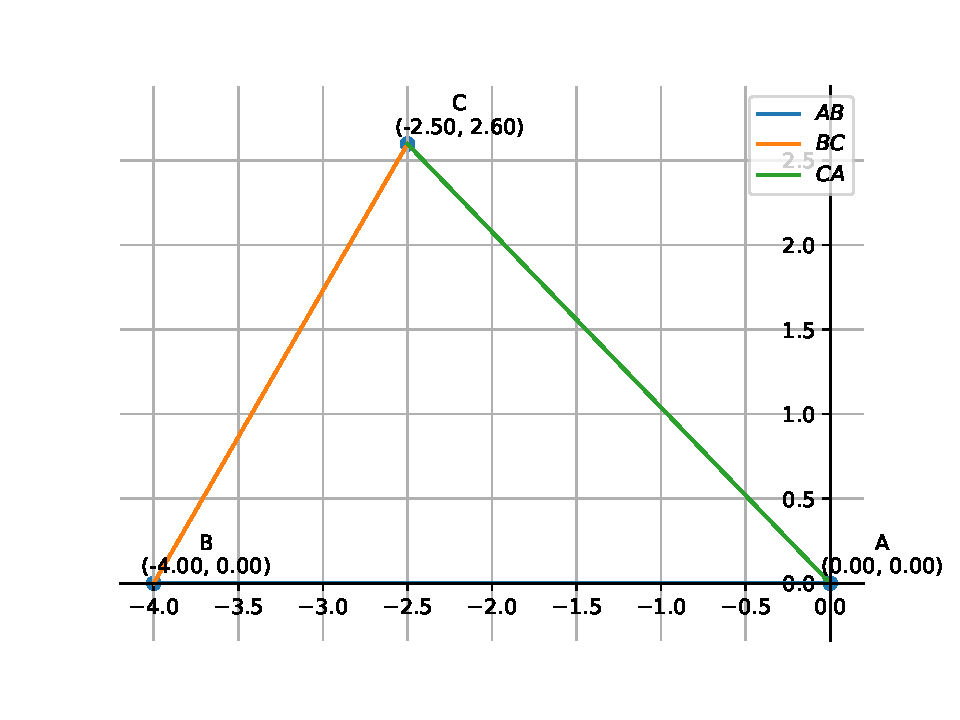
\includegraphics[width=0.75\columnwidth]{chapters/12/10/5/3/figs/fig.pdf} 
 \end{center} 
\caption{} 
\label{fig:chapters/12/10/5/3Fig1} 
\end{figure}
